\chapter{Implementation}\label{sec:implementation}

This section goes over the solutions and implementation that were selected over the course of the semester project. \\

To ensure clarity, this part will be keeping with the three-module  structure established in the previous chapter. 

\section{The Choreographer Application - User Experience}

\begin{figure}[ht]
   \centering
   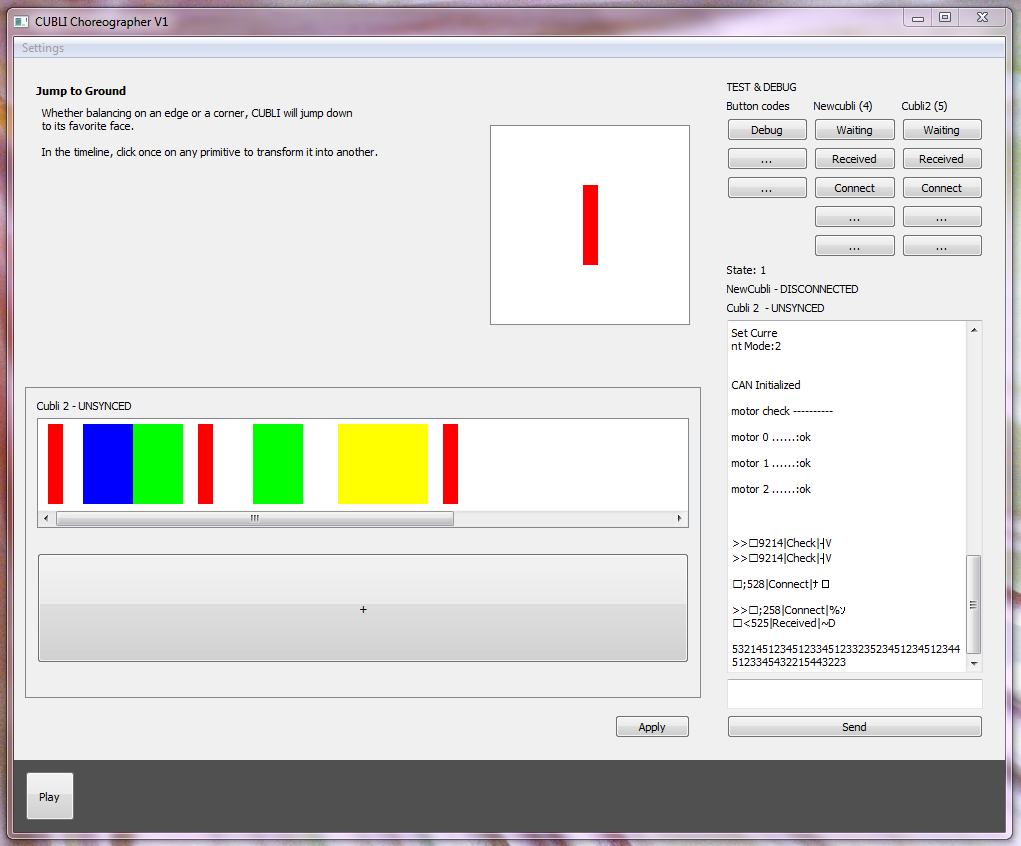
\includegraphics[width=0.75\textwidth]{img/ChoreographerGUI.png}
   \caption{The CUBLI Choreographer Graphical User Interface.}
   \label{img:ChoreographerGUI}
\end{figure}

In the end the choreographer application is quite close to the initial concept. Whereas one could have expected it to evolve differently, the first approach has remained a valid implementation during the project and thus the concept has not deviated much from the outset.\\

One notable addition is the creation of a debugging panel, to the right of the main window, which can also be completely deactivated and hidden. When it is visible however, it provides access to all the communications, and to manually send out messages from the computer, or to simulate incoming messages from cubes.\\

\begin{figure}[ht]
   \centering
   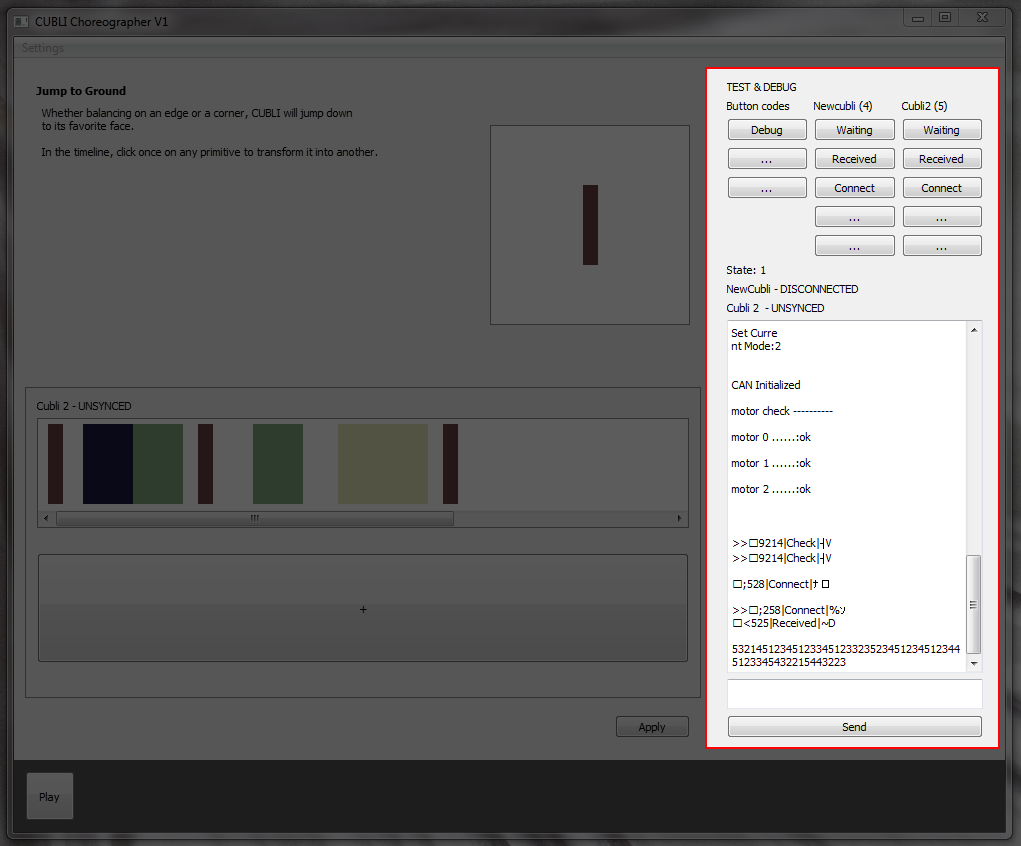
\includegraphics[width=0.75\textwidth]{img/DebugPanel.png}
   \caption{The debugging \& information panel.}
   \label{img:DebugPanel}
\end{figure}

\subsection{Language}

C++ was the obvious choice for a language for three reasons: i) it allowed to reuse code structure from the C source with few modifications ii) the communication protocol could be compiled on the two different machines from the same C file, thus greatly reducing the chances of bugs appearing due to unvoluntary divergences in the protocol source code iii) On the first targeted machine, it had readily available libraries for all the necessary peripherals and UI elements, as well as useful object-oriented features. 
The libraries in question were taken from the QT development kit, a decision which was not obvious as the advantages of QT over Visual Studio appear marginal. \\

Just as the final application, in debugging mode, has two main panels - one concerning the user interaction, specifically the creation of timelines and control of the choreography evolution; one displaying communications through the serial port and state machine information - the development process was centered around two features : i) serial port communication and ii) timeline creation, transfer, and execution. 

\subsection{App Components}

Here we clarify the contents of various parts of the choreographer app source, as available in the Github repository. For each part, a general explanation is given, and if any are relevant, is followed by more technical details.

\subsubsection{Main Window}

First and foremost, this class displays and sets up the main viewport. It defines the action for all the buttons, and provides functions for updating text fields such as the app information.

As such it is mostly QT-specific code, with several functions handling the app behavior when connecting or syncing with cubes.

\subsubsection{Serial Manager}

Serial port communication was the first implemented functionality of the app, relatively easy to write thanks to the already well-built QT serial port libraries. In detail, successful sending entails: 

\begin{itemize}
\item setting the port name ( Later, a panel for setting those options easily, which among other things contains a drop down list enumerating the available port names was added ) 
\item setting the serial parameters, such as baud rate, hardware flow control and so on to the same values as inside cubli ( Baud rate of 115200, ) 
\item open the port. This is straightforward through a simple function call 
\item send bytes through the port. A function call is all that is needed here as well. 
\end{itemize}

Receiving is handled in an interrupt, which hands over control to a function written for that purpose.\\

Among other things this function displays all the received bytes in a serial stream display panel. In addition, any bytes sent by the Application over serial are also displayed in the same serial stream display panel with a line prefix of '>>' \\

The class named Serial Manager was created in order to handle those actions. 

\subsubsection{Timeline}

Created and displayed when each cube connects to the application, a white rectangular canvas on which the user can place, modify or remove color coded squares is meant to represent the chorography - the horizontal axis representing time, - and, as such, is called a Timeline. Each square, called a Primitive, represents a specific action of cubli, and thus, one or several Timelines, each containing a sequence of primitives, together represent a choreography. \\

\begin{figure}[ht]
   \centering
   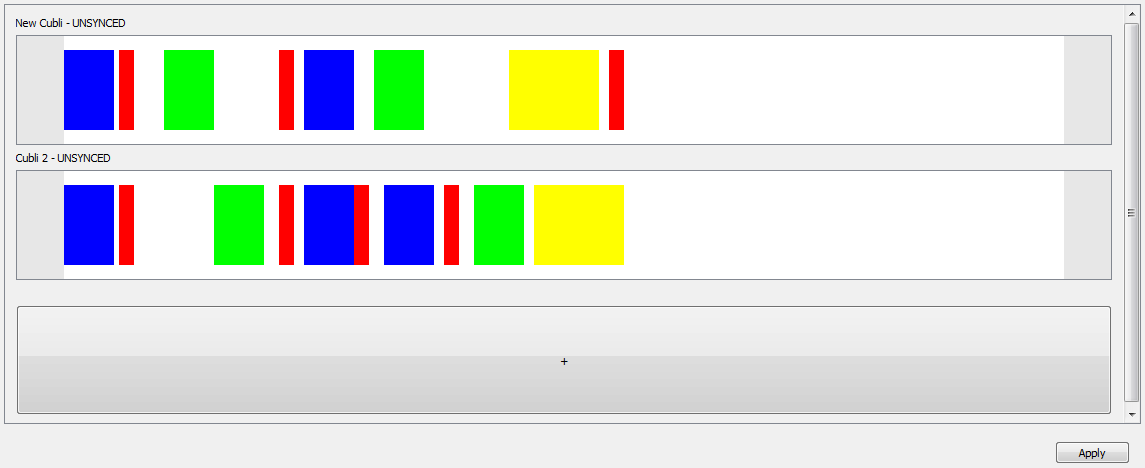
\includegraphics[width=0.75\textwidth]{img/TimelinesPanel.png}
   \caption{The Timeline Editor panel.}
   \label{img:TimelinesPanel}
\end{figure}

For this purpose, within this projet the timeline canvas, or "Graphics Scene" in QT nomenclature, was programmed to respond to user interactions in the following ways: 
\begin{itemize}
\item Clicking on empty space creates a new primitive at that position 
\item Clicking a primitive modifies it, cycling through the available types one at a time 
\item Double clicks are no different from two simple clicks 
\item Left click-and-dragging a primitive moves it based on mouse position 
\item Right clicking a primitive erases it 
\item Right click-and-dragging erases all primitives under the cursors path 
\item Left click and dragging on empty space has no effect 
\end{itemize}

\subsubsection{Timeline - Technical Addendum}

QT allows the interception of mouse events inside the Timeline area through several functions, of which \texttt{MousePressEvent(), MouseMoveEvent(), MouseReleaseEvent(),} and \texttt{MouseDoubleClickEvent()} are used here. Each one of these functions is executed upon the appropriate event, \texttt{MousePressEvent()} in particular gets triggered by both left and right mouse clicks.  \texttt{MouseDoubleClickEvent()} replaces \texttt{MousePressEvent()} when the relevant click is second in a series.

Programmatically this behavior was encoded as follows: 

\begin{itemize}
\item[] \texttt{MousePressEvent()}: When a mouse button is pressed within the timeline bounds, the application checks whether a primitive is present under the cursor. In the case that the right mouse button was pressed, the primitive under the cursor is immediately deleted. Otherwise, the primitive under the cursor, if any, is simply marked ( "selected" ) for later. No further action is undertaken until another mouse event occurs. 
\item[]  \texttt{MouseMoveEvent()}: If a primitive is currently selected, it follows the position of the cursor, as far as collisions allow it.
\item[]  \texttt{MouseReleaseEvent()}: If a primitive is currently selected and no mouse movement was made, it is transformed into the next primitive type. If a primitive is currently selected and mouse movement was made, its type remains unchanged. If no primitive was selected, a new one is created. The primitive information panel is updated to reflect the latest selected or created primitive, and any selected primitive is unselected.
\item[]  \texttt{MouseDoubleClickEvent()}: In order to stay consistent with single click behavior, this function does exactly what a \texttt{MousePressEvent()} does.
\end{itemize}


\subsubsection{Primitive}

The primitive class is an extension of simple rectangle objects in the timeline, adding extra properties such as type, and automatically assigning styles, width, or positions, thus making them simpler to display and move around. These extended rectangle objects are meant to visually represent the action primitives of a cube in the choreography.\\

This class provides methods for easily accessing certain properties, modifying, or moving the primitives around, for example without running into each other.

\subsubsection{ComStateManager}

 The ComStateManager class is the part of the application which handles communication responses, i.e. \textit{what to send and when}.\\
 
Any message sent to the cube from the app means a call to this class. It is also where cube statuses are stored, which allow it and other parts of the application to take into account whether particular cubes are connected or not, syncing or not, and so on.\\

Which message must be sent is necessarily determined in this class' logic.
It accomplishes this through a state machine, that has a corresponding response for every incoming message or application call.\\

The protocols described in the next section are mostly encoded in here ( messages which are sent several times in a row originate from \texttt{mainwindow.cpp} code )

\subsubsection{SettingsDialog}

SettingsDialog is responsible for putting together the settings dialog which appears when the serial port settings are to be modified, and storing their values.

\subsubsection{Main.cpp}

Main runs the mainwindow code, launching the app, and any necessary QT routines.

\section{Communications}

The source for the message protocol fits inside one cpp file and accompanying header. It mainly creates or deconstructs strings or characters, in order to transmit and receive messages which satisfy the required specifications.\\

Of course, the concept of communication protocol as a whole pertains to more than uniquely this message-transmission code. It also englobes the determination of how the machines ought to behave when contacting each other, which in practice is encoded all over their code ( see communication state machines, MainWindow, etc ). However for the sake of consistency the particulars of these protocols are discussed here.\\

One of the difficulties during this project was the unreliability of the UART behavior in the cubli microcontroller ( \textit{See Figure \ref{img:USART}} ). Thankfully the communication protocol was designed to be quite robust from the get-go, which seemed at the time like a potentially unnecessary amount of safety, though it proved essential.

\begin{figure}[ht]
   \centering
   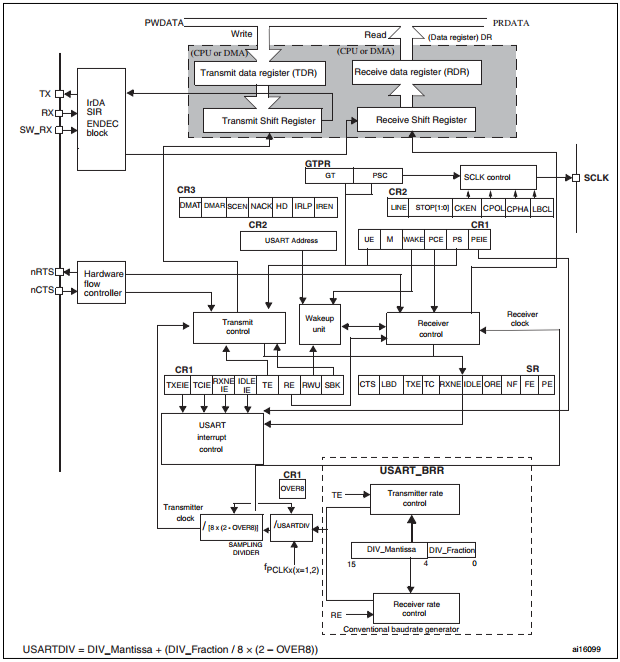
\includegraphics[width=0.75\textwidth]{img/USART.png}
   \caption{USART Block diagram as shown in \cite{stm32manual}.}
   \label{img:USART}
\end{figure}

The inability to work with the assumption that 'the majority of messages would be able get through successfully' also meant that communication protocols were not simply a formality, and had to be designed with contingencies in mind. This made this module an interesting, though larger than anticipated, part of the project.

\subsection{com\_protocol}

Principally, this code transforms a message's code, additional content, and metadata into a normalized string of characters which can be sent one byte at a time over UART. And vice-versa.\\

It is here that the structure of a message is defined, and this code applies to both Cublis and the choreography application.\\

This message structure is as follows:
\begin{itemize}
\item[] Messages begin with a \textbf{start-byte}. This allows the code to more efficiently decrypt messages among garbage bytes in a buffer.
\item[] The \textbf{message length} is encoded in the next byte, so as to allow the decryptor to know where the message ends.
\item[] The next two bytes are, respectively, the \textbf{sender ID} and \textbf{recipient ID}.
\item[] Then comes the \textbf{message code}, first part of a message's actual content.
\item[] Second part of the message's content, are three potential \textbf{extra-content} bytes.
\item[] If the verbose flag is set, a \textbf{human-readable description} of the message and extra-content is inserted at this point.
\item[] The last two bytes of every message encode the \textbf{hash}, used for verifying message integrity. When decrypting messages, bits are mixed together according to a common algorithm, and the result is compared to the hash bytes carried by the message. Should they not match, the message is discarded.
\end{itemize}

\textit{See Figure \ref{img:Message} for an example of a valid message.}\\

\textbf{Note:} When the COM\_VERBOSE compile flag is defined message length, message codes, sender and recipient IDs are increased by 48 - the ASCII value for the character '0'. This is performed for ease-of-use: while smaller than 10, their values are human readable when the message is in ASCII form. 

\begin{figure}[ht]
   \centering
   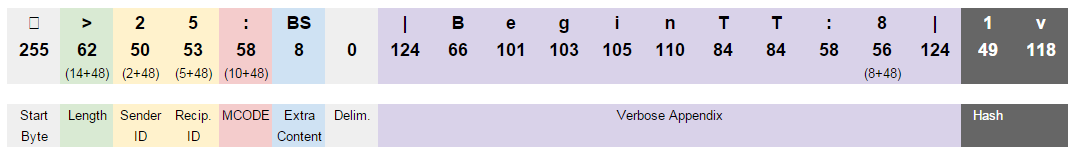
\includegraphics[width=0.75\textwidth]{img/Message.png}
   \caption{Decomposition of an example message, created with the COM\_VERBOSE compile flag defined.}
   \label{img:Message}
\end{figure}

\subsubsection{Header}

The header, com\_protocol.h contains enumerations for all the message codes, communications states, and a few other which are shared between cubli and computer, as well as some macro expansions which concern communication settings.\\

\textit{Message Codes}\\

Message codes are defined as an enumeration, and are automatically assigned integer values. \textit{See Table \ref{tab:mcodes}}.\\

\begin{table}[ht]
\begin{center}
\caption{Message codes and their string labels, as defined in \texttt{com\_protocol.h} and \texttt{com\_protocol.c}.}\vspace{1ex}
\label{tab:mcodes}
\begin{tabular}{ll}\hline
Message Code & Corresponding String ( Verbose ) \\ \hline 
COM\_MCODE\_NOTHING             & "|"                  \\
COM\_MCODE\_NOMESSAGE           & "|?"                 \\
COM\_MCODE\_ERROR               & "|Error"             \\
COM\_MCODE\_WAITING             & "|Waiting"           \\
COM\_MCODE\_CHECK               & "|Check"             \\
COM\_MCODE\_RECEIVED            & "|Received"          \\
COM\_MCODE\_RECEIVED\_PART      & "|Received:"         \\
COM\_MCODE\_SHUTDOWN            & "|Shutting Down"     \\
COM\_MCODE\_CONNECT             & "|Connect"           \\
COM\_MCODE\_DISCONNECT          & "|Disconnect"        \\
COM\_MCODE\_BGN\_SND\_TMLN      & "|BeginTT:"          \\
COM\_MCODE\_END\_SND\_TMLN      & "|FinishTT"          \\
COM\_MCODE\_ABORT\_SND\_TMLN    & "|AbortTT"           \\
COM\_MCODE\_SND\_TMLN\_PART     & "|TTData:"           \\
COM\_MCODE\_COUNTDOWN           & "|Start in:"         \\
COM\_MCODE\_GOT\_COUNT          & "|Got count"         \\
COM\_MCODE\_STARTED             & "|C'est parti!"      \\
COM\_MCODE\_SUCCEEDED           & "|Move successful"   \\
COM\_MCODE\_FAILED              & "|Move failed"       \\
COM\_MCODE\_ACCUSE              & "|Other cube failed" \\
COM\_MCODE\_STUCK               & "|Failed and stuck"  \\
COM\_MCODE\_ACKNOWLEDGE         & "|Acknowledged"      \\
COM\_MCODE\_RECOVERED           & "|Recovered"         \\
COM\_MCODE\_STOP                & "|Stop Performance"  \\
COM\_MCODE\_RESUME              & "|Resume in:"        \\
COM\_MCODE\_FINISHED            & "|Ended Performance" \\
COM\_BCODE\_CHECK\_CUBES        & "|BCODE"             \\
COM\_BCODE\_START\_IN           & "|BCODE"             \\
COM\_BCODE\_STARTED             & "|BCODE"             \\
COM\_BCODE\_TRANSFER            & "|BCODE"             \\
COM\_BCODE\_ABORT\_TRANSFER     & "|BCODE"             \\
COM\_BCODE\_ABORT\_PERFORMANCE  & "|BCODE"             \\
COM\_BCODE\_RESUME\_PERFORMANCE & "|BCODE"             \\
COM\_MCODE\_DEBUG               & "|DEBUG"             \\
COM\_N\_MESSAGE\_CODES          & [Not a valid code]  \\
 \hline
\end{tabular}
\end{center}
\end{table}

BCODEs, short for Button Codes, are message codes which are internal to the choreographer application. They are used to convey button inputs or events to the communications state machine, and are not meant to be transmitted over UART.\\


\textit{Compile flags}\\

The header also contains two compile flags:\\

\begin{itemize}
\item[] COM\_VERBOSE

	if this flag is defined, messages also contain a human-readable appendix expliciting the relevant message code, and extra content. By default, this flag is defined.

\item[] COM\_DEBUG

	if this flag is defined, extra information pertaining to failure when decrypting messages is displayed as plain text. This is for example useful when messages are not getting decrypted though they are transmitted correctly. By default, this flag is not defined.
    
\end{itemize}

\subsection{Information Reception \& Decryption}

The way Cublis and the choreographer application handle UART information is similar, although there are specific details that differ.\\

The step-by-step process of reception and decryption in both device types is as follows:\\

\begin{itemize}
\item At the lowest level, and on every device, all bytes emitted over UART are immediately captured and stored into a buffer - whether they are part of a message or not. The only exception, of course, are the bytes which fail to transmit for one reason or other.

\begin{description}
\item[In Cubli,] the buffer in question is a ring buffer named \textit{rx\_buf}. The interrupt routine \textit{USART1\_IRQHandler()} checks whether a byte has been stored in the UART register. If it has, it places the byte into \textit{rx\_buf} and empties the UART data register. Over time, the buffer fills up with sequences of bytes, and stops storing them when full. Since these interrupts are designed to be as light as possible, the actual emptying, and reading of the buffer has to be done somewhere else. In this case, the ComManagement task is responsible for that among other things, and does so in a periodic manner.
\item[In the Choreographer,] similar behavior is implemented in appropriate libraries. At this point, the aspect which differs from the cubli implementation is that these libraries are configured to immediately handle data after a burst of bytes is received - i.e. a call is made to the function \textit{readData()} after every group of bytes which are sent in quick succession. \textit{readData()} contains the next step in handling and decryption of the information.
As such, cubli performs the next step periodically, while the choreographer app does so in a responsive manner.
\end{description}

\item Next, the data present in the low-level buffers described above are appended to a second, higher-level buffer, which is accessed less often. The contents of this second buffer are passed to the \textit{decrypt\_message()} function in com\_protocol.c. If a message is present in these contents, it is disassembled, and verified. If a message is not intended to have the current device as a recipient, it is discarded. If its length or hash is invalid, it is also discarded.

\begin{description}
\item[In Cubli,] this step is done inside the ComManagement task. Particularities are: the buffer is erased and overwritten on every loop of the task, instead of having the new data appended to it. This is due to the fact that testing of the append-data method yielded worst results, against expectations. \textit{ It is hypothesised that the period of the ComManagement task being larger than the time it takes for the choreographer to emit an entire sequence of bytes composing a message, and that length of time being extremely small, chances of messages being separated is very low. Low enough that the append-data method's advantage, that is, reconstitution of separated messages, is not significant enough to compensate the performance loss due to increase in task complexity.}
\item[In the Choreographer,] data is appended on the high-level buffer, thus separated messages are reconstituted. This was shown to have a significant positive impact, as the likelihood of messages being separated upon reception by the choreographer app is higher - likely due to the event-based nature of the choreographer UART data handling.
An interesting point is the fact that as soon as the first message present in the buffer is read ( more precisely, if \textit{decrypt\_message()} returns a non-zero value ), the entire buffer is cleared and any messages already present in the remaining bytes is thus thrown away. This was done to keep up with the high communication frequency that can arise - in the case where messages are emitted too fast, if the app were to treat every single one it would progressively lag behind ( this has been tested, and is effectively the case ). 
\end{description}

\item At this point, the devices can handle the decrypted message, thanks to their appropriate communication state machines. 

\begin{description}
\item[In Cubli's case,] the absence of any data, or the presence of data which does not contain a valid message are also handled. This is useful as a consequence of the periodic aspect of the ComManagement task. 
\item[In the Choreographer,] button or interface events can also be passed to the state machine, in order to have communication responses to those inputs.
\end{description}

\end{itemize}

\subsection{Protocols}

The protocols which determine the communication behavior of every device are strongly dependent on the situation, more precisely the state in which a device is. \\

This is due to the significant transmission failure rate experienced during the project. 

Such a transmission rate means that not every desired aspect of a program can be attained, and the type of protocol used determines which aspect is impacted most when transmissions fail. Each situation had different critical aspects which needed to be prioritized, thus the protocols had to be adapted accordingly.\\

In this report, a \textit{communication protocol} refers to the rules of communication between devices, which state what the standard procedure is in a back-and-forth exchange of information, and all alternate procedures if at any point a message fails to transmit.\\

Such a standard procedure can for example be explicited as follows:
\begin{itemize}
\item[] \textbf{A to B:} "start of protocol"
\item[] \textbf{B to A:} "confirmation"
\item[] \textbf{A to B:} "end of protocol"
\end{itemize}

when all involved parties have received their intended messages, the protocol is considered as having completed successfully.\\

Alternate procedures describe the prescribed response when a message from the standard procedure is not delivered as intended.

\subsubsection{In General}

Some proprieties of the communication protocols created for this project are generally true.\\

The last message of any protocol procedure is a sensitive one, as there is nothing in the procedure itself that allows the emitting party to be aware of whether the receiving party has successfully collected it ( if an extra confirmation is added for this purpose, this confirmation becomes the last message of the protocol, and the same issue applies once again. And so on. ). \\

It is therefore to be expected that one device, having not received the ultimate message of the protocol procedure, is still expecting/asking for it, while the other device, having sent it, considers the protocol procedure completed.
In that case, or if for any other reason one device remains stuck in procedure while the other one does not - e.g. if one of the two is reset unexpectedly - it is necessary to implement general or specific protocol-aborting procedures.\\

For example the use of a timeout allows such a stuck-device to exit the procedure by itself after a while. Illustrated:

\begin{itemize}
\item[] \textbf{A to B:} "start of protocol"
\item[] \textbf{B to A:} "confirmation"
\item[] \textbf{A to B:} "end of protocol" \textbf{not delivered, A exits protocol.}
\item[] \textbf{B waits...}
\item[] \textbf{timeout: B exits protocol.}
\end{itemize}

The stuck device can also periodically ask for the last message to be re-sent, as long as it has not received it. As a complement to this process, a timeout can be implemented to prevent infinite loops. Illustrated:

\begin{itemize}
\item[] \textbf{A to B:} "start of protocol"
\item[] \textbf{B to A:} "confirmation"
\item[] \textbf{A to B:} "end of protocol" \textbf{not delivered, A exits protocol.}
\item[] \textbf{B waits...}
\item[] \textbf{B to A:} "confirmation"
\item[] \textbf{B waits...}
\item[] \textbf{B to A:} "confirmation"
\item[] \textbf{B waits...}
\item[] \textbf{timeout: B exits protocol.}
\end{itemize}

Otherwise, or in addition, devices having already exited the protocol can be programmed to respond to tell-tale "second-to-last messages" with the correct protocol terminating message, without themselves being in the same state. Illustrated:

\begin{itemize}
\item[] \textbf{A to B:} "start of protocol"
\item[] \textbf{B to A:} "confirmation"
\item[] \textbf{A to B:} "end of protocol" \textbf{not delivered, A exits protocol.}
\item[] \textbf{B waits...}
\item[] \textbf{B to A:} "confirmation"
\item[] \textbf{X to B:} "end of protocol"  \textbf{B exits protocol.}
\end{itemize}


\subsubsection{Connecting Protocol}

The choreographer application needs to know which cubes are connected, and which aren't. This is in order to spare the user the necessity of manually adding and removing cubes, as well as the potential errors that come with it ( mislabeled cubes, non-existant cubes, ... ). Cublis, however, have no need to know whether they are connected or not - the app either sends them commands and information, or it does not.

As a result, the connection protocol is not symmetrical. 

\begin{description}
\item[Standard protocol procedure]:

\begin{itemize}
\item[] \textbf{Cubli to PC:} "connect"
\item[] \textbf{PC to Cubli:} "connect"
\item[] \textbf{Cubli to PC:} "received"
\end{itemize}

at which point, the application changes the appropriate cubes status to "Unsynced"
\item[Alternate procedures]:

Cubli periodically repeats the first message until it receives confirmation, i.e. a "connect" message from the application. It tries approximately 10 times then aborts the procedure. \textit{"Approximately" in the previous sentence points to the fact that Cubli can try up to a 100 times, the exact amount of times depends of wether it receives in return an undecypherable message, or nothing at all.} Illustrated:

\begin{itemize}
\item[] \textbf{Cubli to PC:} "connect" \textbf{not delivered}
\item[] \textbf{Cubli to PC:} "connect"
\item[] \textbf{PC to Cubli:} "connect" \textbf{not delivered}
\item[] \textbf{Cubli to PC:} "connect"
\item[] \textbf{PC to Cubli:} "connect" 
\item[] \textbf{Cubli to PC:} "received"
\end{itemize}

Should the ultimate message not be delivered, or should cubli give up, the procedure is incomplete from the application's point of view, and needs to be initiated again. No extra procedure was implemented to prevent this, as the occurrence is rare and re-initiating the procedure is not problematic.


\item[Also]:

The application can prompt cubes to initiate this protocol, by sending the "check" message to all cubes. Cubes which receive it send a "connect" message in return, first message in the procedure. In order to maximize the chances of all cubes initiating the procedure, the choreographer application sends 10 "Check" messages during a period of one second.


\end{description}

\subsubsection{Sync Protocol}

The application performs the same procedure for each connected cubli, one after the other. It goes as follow:

\begin{description}
\item[Standard protocol procedure]:

\begin{itemize}
\item[] \textbf{PC to Cubli:} "begin transfer : 5 parts"
\item[] \textbf{Cubli to PC:} "received"
\item[] \textbf{PC to Cubli:} "part 1"
\item[] \textbf{Cubli to PC:} "part 1 received"
\item[] \textbf{PC to Cubli:} "part 2"
\item[] \textbf{Cubli to PC:} "part 2 received"
\item[] \textbf{idem. for parts 3 to N ...}
\item[] \textbf{PC to Cubli:} "part N"
\item[] \textbf{Cubli to PC:} "part N received"
\item[] \textbf{PC to Cubli:} "finish transfer"
\item[] \textbf{Cubli to PC:} "received"
\end{itemize}

\item[Alternate procedures]:

The first message is resent by the application until confirmation of reception.

From that point on, every 50ms during which cubli does not receive a part, it sends a "waiting" message. 
Upon reception such one "waiting" message, otherwise periodically, the application re-sends the latest part or "finish transfer" message. It does so until a timeout is reached, at which point the application sends 10 "abort transfer" messages, and disconnects the cube if it has not mirrored any of the 10 "abort transfer" messages.

The cube has no timeout, and should a cube for any reason remain stuck sending out "waiting" messages, the app is programmed to respond with "abort transfer" if is not, itself, in the sync state.

\end{description}

\subsubsection{Choreography Start Protocol}

\begin{description}
\item[Standard protocol procedure]:

\begin{itemize}
\item[] \textbf{PC to Cublis:} "start in: 10"
\item[] \textbf{Cublis to PC:} "got count"
\item[] \textbf{PC to Cublis:} "start in:  9"
\item[] \textbf{Cublis to PC:} "got count"
\item[] \textbf{PC to Cublis:} "start in:  8"
\item[] \textbf{Cublis to PC:} "got count"
\item[] \textbf{idem. from 7 to 2...}
\item[] \textbf{PC to Cublis:} "start in:  1"
\item[] \textbf{all devices start choreography}
\end{itemize}

Every cubli has 7 chances to receive and confirm the countdown. If the PC does not receive at least one confirmation from each cubli by the time the countdown reaches 3, it marks the offending cubli as disconnected, and begins the Abort Choreography protocol.

\end{description}

\subsubsection{Abort Choreography Protocol}

\begin{description}
\item[Standard protocol procedure]:

\begin{itemize}
\item[] \textbf{PC to Cublis:} "stop choreography"
\item[] \textbf{Cublis to PC:} "stop choreography"
\end{itemize}

The PC repeats the message 10 times, or until it has received at least one confirmation from each cube. Should no confirmation be received from one cube, it is marked as disconnected.

\end{description}

\subsubsection{Choreography Failure Protocol}

\begin{description}
\item[Standard protocol procedure]:

\begin{itemize}
\item[] \textbf{Cubli A      to All:} "move failed"
\item[] \textbf{PC       to Cubli A:} "acknowledged"
\item[] \textbf{Other Cublis  to PC:} "other cubli failed"
\item[] \textbf{PC  to Other Cublis:} "acknowledged"
\item[] \textbf{all devices wait for recovery}
\item[] \textbf{Cubli A       to PC:} "recovered"
\item[] \textbf{PC       to Cubli A:} "acknowledged"
\item[] \textbf{PC           to All:} "resume in 10"
\item[] \textbf{All Cublis   to PC :} "resume in"
\item[] \textbf{PC           to All:} "resume in  9"
\item[] \textbf{All Cublis   to PC :} "resume in"
\item[] \textbf{PC           to All:} "resume in  8"
\item[] \textbf{All Cublis   to PC :} "resume in"
\item[] \textbf{idem. from 7 to 2...}
\item[] \textbf{PC           to All:} "resume in  1"
\item[] \textbf{All Cublis   to PC :} "resume in"
\item[] \textbf{all devices resume choreography}

\end{itemize}

[Alternatives]

\end{description}

\section{Cubli Development}

In order to avoid introducing new bugs, care was taken to build on top of already-existing functionality rather than to modify it, as much as possible.

This means that except for a few additional line of codes, the controllers remain unchanged, and the code relevant to this project is composed of additional tasks for communication, choreography, and additions in mode management.\\

These relevant parts are what will be discussed here, rather than the entire cubli source code.

\subsection{Refresher: Cubli Source Code }

Before the project additions are described, it is useful to understand how the already-existing Cubli code handles inputs and events, as well as its general structure.\\

The main routines executed inside cubli softwares are managed by a realtime OS, which compartimentalizes them into various tasks, giving to each their respective processor access time, depending on their priority, period, and so on. This allows several processes to run in parallel, without necessarily affecting each other.\\

As an example, some tasks in the cubli source code are responsible for regularly checking that user inputs have been made, while others are responsible for the high-frequency control necessary during movements, such as the LQR controller task for balancing.\\

In addition, the OS also deals with interrupt routines and more specific functions outside of tasks, of which only the UART interrupt routine and button-press event handler are relevant to this report.\\

\subsubsection{From Button Press to Edge Balance}

\begin{itemize}
\item In \textbf{stm32f4xx\_it.c}, an interrupt is triggered when the mode button is pressed. Inside this interrupt, the \texttt{ \_modeNumber } variable is incremented once.

\item In \textbf{Controllers.c}, the ModeManagement task is repeated every few milliseconds. On every loop, it checks whether the mode number has changed - and whether the ReRunModeManagement variable has been set. If either of those conditions are true, it measures what position Cubli is currently in, and updates the controller task management variables accordingly - based on the current new mode number.\\

\textbf{Furthermore :} 
\begin{itemize}
\item[] Before updating those variables, it checks that the mode number was not changed two consecutive times in short order - indicating an involuntary double button press.
\item[] ReRunModeManagement is triggered inside ModeManagement, when cubli is set on its face. This is done order to re-update the controller task management variables - i.e. restart the current action. 
\item[] Following this, ModeManagement waits 5 seconds before updating the controller task management variables, in order to prevent immediate and ill-controlled behavior.
\end{itemize}

\item Still in \textbf{Controllers.c}, the task management variables, \texttt{\_jumpMode, \_balance, \_balancingMode} determine whether controller tasks execute actions or wait idly. These tasks access IMU and sensor measurements, calculate the necessary control actions, and set target actuation values appropriately. Actuation tasks then attempt to realize those values and interact with the servo hardware.
\end{itemize}

See Figure \ref{img:Controllers} for a visual overview of this process.

\begin{figure}[ht]
   \centering
   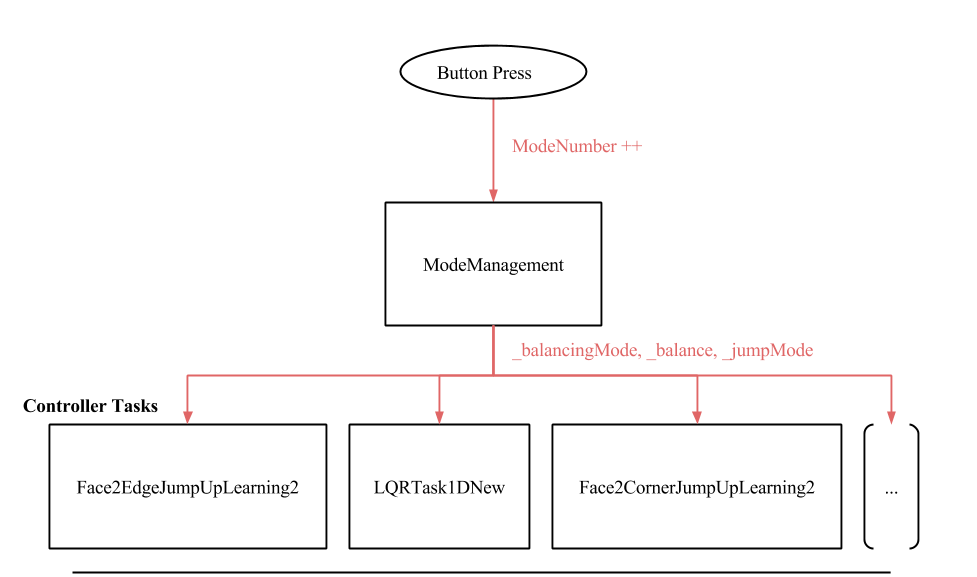
\includegraphics[width=0.75\textwidth]{img/Controllers.png}
   \caption{Block diagram of tasks in the original \texttt{Controllers.c}, illustrating the control flow for move executions.}
   \label{img:Controllers}
\end{figure}


\subsection{Task Alterations}

The bulk of the additions to the Cubli code affected tasks, with the modification of several existing tasks, and creation of 2 new tasks for communication and choreography management.\\

This subsection describes the code modifications and additions to the relevant tasks performed in this project.\\

See Figure \ref{img:ControllersChoreography} for an overview of the resulting task interactions.

\subsubsection{ModeManagement Task}

Originally a task responsible for updating the global variables responsible for deciding which controllers get activated based on the current mode ( which is originally incremented through the press of a respective hardware button ), this functionality is conserved and extended in this project.\\

New modes are created for choreography, corresponding to the movement primitives, while the original modes are renamed to button modes, and relevant code sections are modified to make the new and original modes cohabitate. To this end, the original and old modes are distinguishable, allowing behavior which was only needed in old modes to be disabled for the new modes only.\\

[Old modes and New Modes]\\

[Pause upon resetting cubli on face?]\\

\subsubsection{ComManagement Task}

Created during this project, the ComManagement task contains both the code responsible for reading from the UART buffer, and a communication state machine similar to the one in the choreography app.\\

One notable difference between the communication behavior of cubli compared to the app is that its communication state machine is triggered regularly rather than on specific event occurences. This is discussed in further details inside this chapter's \textit{Communications} section, in the \textit{Information Reception \& Decryption} subsection.\\ 

As for the communication state machine, it implements the protocols which are described inside this chapter's \textit{Communications} section, in the \textit{Protocols} subsection. 

\subsubsection{ChoreographyManagement Task}

The choreography management task is only active during choreography, in which case it keeps track of the current primitive and run time, and adjusts the mode accordingly. It also implements behavior for pausing the choreography and notifying other cubes through the communication management when a move fails.

\subsubsection{TimelineStatus Task}

This code is responsible for storing the timeline information.\\

A cube stores only one timeline, its current timeline, which it does not modify. Alongside it, is a 'cache', a temporary timeline which is filled during sync, and then copied to the current timeline if the sync was successful, or discarded if unsuccessful.\\

[Limits of timeline storage, etc]

\subsubsection{Controller Tasks}

Some controller tasks were modified, to the smallest necessary extent, to fit with the choreographer functionality. Care was taken to ensure that the controller behavior would remain unchanged outside of choreography (i.e. with the relevant code sections being bypassed by if-clauses checking for choreography activity)

Three functionalities had to be added in the controllers' code:
\begin{itemize}
\item the ability for cubli to fall down to a face on its own
\item regulating the braking time to help synchronize choreographies
\item notifying the choreography management task when primitives are successful
\end{itemize}

\begin{figure}[ht]
   \centering
   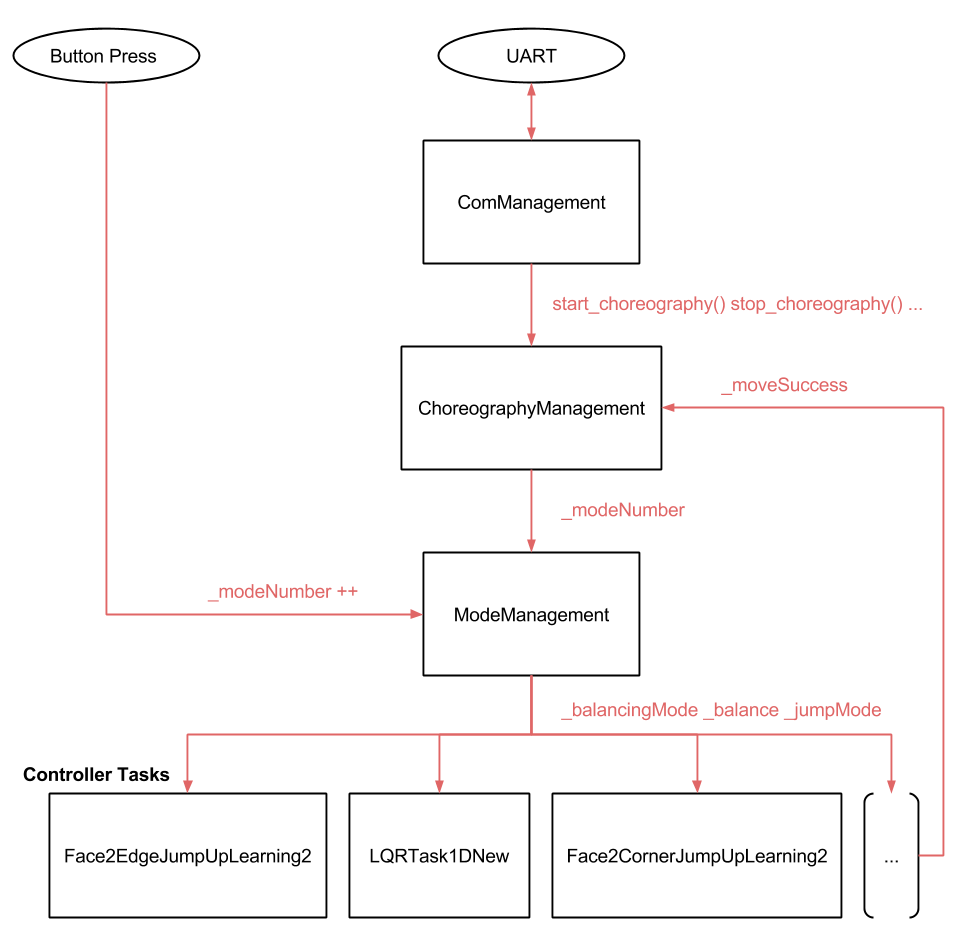
\includegraphics[width=0.75\textwidth]{img/ControllersChoreography.png}
   \caption{Block diagram of tasks in this projects' updated \texttt{Controllers.c}, illustrating the control flow for move executions.}
   \label{img:ControllersChoreography}
\end{figure}

\subsection{Other Alterations}

UART routine

Button-press event


    



